\documentclass[conference]{IEEEtran}
\usepackage{amsmath,amssymb,booktabs,graphicx,xcolor}
\usepackage[hidelinks]{hyperref}
\usepackage{url}
\usepackage{balance}
\usepackage{iftex}
\ifXeTeX
\usepackage{fontspec}
\setmainfont{texgyretermes-regular.otf}[BoldFont=texgyretermes-bold.otf,ItalicFont=texgyretermes-italic.otf,BoldItalicFont=texgyretermes-bolditalic.otf]
\setsansfont{texgyreheros-regular.otf}[BoldFont=texgyreheros-bold.otf,ItalicFont=texgyreheros-italic.otf]
\setmonofont{texgyrecursor-regular.otf}[BoldFont=texgyrecursor-bold.otf]
\fi
\title{Maintaining Source-Linked Evidence Views for Agent Memory}
\author{\IEEEauthorblockN{Anonymous authors}}
\begin{document}
\maketitle
\begin{abstract}
A coding agent proposes a file to read, a tool withdraws a previous dependency, and an edit moves lines the agent read earlier. Which addresses can a memory store return, and what evidence still supports them? We demonstrate a local SQLite system for maintaining and auditing three views: a ranked source, a token-budgeted packet, and a set of code spans. A visitor can promote a proposed file to an observed read, rewind an actual edge withdrawal, or compare preserved code lines against the next snapshot. On 1,112 trace states, histories returned the same addresses and scores as fresh reconstruction. A rank-bound certificate recomputed the full top eight by index on only 39 of 1,072 updates, with similar warm latency to a simpler control. In a separate physical comparison a packed top-eight snapshot took 175\,ms versus 218\,ms for membership intervals at eight reads per update. Across 1,071 observed coding-agent edits, local line alignment preserved 323 complete packets versus 302 for range invalidation. On 283 archived coding-agent sessions, proposals yielded 20 additional relevant reads versus 26 for an embedding retriever. The demonstration exposes both the maintenance savings and the limits of using a recorded relation to select useful context.
\end{abstract}

\section{What survives a change?}
A coding agent finishes searching a repository with several open files and one suggested path. Crediting it with the path's contents before the read confuses intention with observation. Even previously read evidence can change: a tool retracts a dependency or an edit moves source lines. Can a database return the evidence that fresh computation would select at a given revision? Does that evidence help given a fixed read budget?

A prior ICDE demonstration, TAPE~\cite{tape}, organizes personal memory as a temporal graph. MemTrace~\cite{memtrace} studies the validity of source anchors at restore time. In repository context retrieval, Agent Retrieval Bench~\cite{arb} distinguishes the files returned by a retriever from those a logged agent actually inspects. Incremental top-$k$ maintenance~\cite{topk} offers algorithms for updating ranked views as data change. Our demonstration brings these questions together in a database interface: each selected item identifies its source, the visitor can alter its availability at one revision, and an independent query can reconstruct the result. We isolate the maintenance question from relevance with separate audit tables and equal-budget retrieval experiments.

\begin{table}[t]
\centering\small
\caption{Source identities retained by the serving database. Each row identifies the observation that can be checked at read time.}
\begin{tabular}{@{}p{.21\columnwidth}p{.32\columnwidth}p{.36\columnwidth}@{}}\toprule
Object & Identity & Receipt or witness\\\midrule
Proposed path & Session, base commit, path & Chunk line range and digest after a read\\
Support edge & Trace, producer, consumer & Before/after weights at a revision\\
Evidence unit & Event, field, character interval & Source IDs, selection rank, utility, cost\\
Code block & File revision, line coordinates & Line content at the new address\\\bottomrule
\end{tabular}
\label{tab:objects}
\end{table}

\section{Three views and their maintenance}
Each local projection serves typed edges, unit IDs and source coordinates over loopback (Table~\ref{tab:objects}). The selector uses observed edges, names and ranks. A separate auditor checks the returned IDs against reference data. Each workload has its own source chronology.

\subsection{Historical ranked sources}
At trace revision $t$, producer $i$ has score $s_i(t)=\sum_j w_{ij}(t)$, where $w_{ij}$ is the active weight of its relation to consumer $j$. The total order is decreasing score, then increasing producer ID. Source additions and withdrawals enter the same transaction. We update the affected scores, obtain the new leader through a covering index and append a receipt only if the pair (address, score) changed. A historical read finds its most recent receipt at or before $t$. This returns the fresh answer because the winning pair is constant between adjacent boundaries. A historical verifier reconstructs the score from active edge intervals and applies the same total order. An incumbent may survive an update with a different score, so this representation compares both fields.

For a top-$k$ read, define $V_t$ as the first eight eligible (ID, score) pairs in total order and return the requested prefix, $k\in\{2,4,8\}$. A packed history writes one snapshot exactly when $V_t$ changes. Another scheme opens and closes validity intervals for (ID, score) pairs entering or leaving the set of eight. A rank change of a continuing pair requires no interval write. Sorting active pairs at read time reconstructs $V_t$, since every stored pair belongs to this set and the total order is fixed. We also implement ranked positions, rank blocks and a candidate-version covering index. These representations trade history written per change against lookups, filtering and decoding at read time.

A write-side certificate can avoid an indexed top-eight query even when the result changes. Re-rank the previous top eight and the rows touched by the transaction, using their new values and the fixed tie order. If this local result supplies eight rows and its eighth key ranks at least as high as the old eighth key, return it. Every untouched outsider was below the old cutoff and retained its key, so none can displace a returned row. If the old view already held the entire candidate pool, all eligible rows are known locally. When the bound fails, use the covering index. The certificate changes the update path and preserves the packed historical representation.

\begin{table}[t]
\caption{SQLite top-eight histories on 1,072 source commits. Time in ms includes schema creation, updates, reads and checkpoint. Eight reads mix current and historical versions equally.}
\centering\small
\begin{tabular}{@{}lrrr@{}}\toprule
Representation & Opens & 0 reads & 8 reads\\\midrule
Changed packed snapshots & 533 & 92.32 & 175.42\\
Individual rank positions & 1,669 & 92.58 & 188.32\\
Three rank blocks & 883 & 94.52 & 179.57\\
Top-eight membership intervals & 717 & 100.20 & 218.11\\
All candidate versions & 1,669 & 110.06 & 215.65\\\bottomrule
\end{tabular}
\label{tab:top}
\end{table}

\subsection{A budgeted evidence packet}
The reader protects the longest consecutive ranked prefix $H$ costing at most $T$, then maximizes additive utility under the remaining token budget by 0--1 knapsack. Costs, utilities, order and a deterministic tie rule remain fixed during a source exclusion.

Let $P$ be the original packet, $D$ the removed candidate IDs, and $H'$ the protected prefix after deletion. The ordered packet can be reused exactly when
\[
                 D\cap P=\varnothing \quad\text{and}\quad H'\subseteq P.
\]
Deleting a chosen unit or forcing an unchosen unit into the new prefix changes the packet. Otherwise the original prefix survives and can only extend. The old optimum stays feasible, every packet feasible after exclusion was feasible before it, and the fixed tie preference preserves identity. For exact utility arithmetic strict-update dynamic programming prefers absence at the last differing rank.

An inexpensive sufficient certificate indexes the selected units and the first unit beyond the prefix. Touching neither preserves the packet. The boundary matters: with costs $(3,3,1,5)$, utilities $(1,1,3,10)$, budget 8 and prefix threshold 4, removing unselected unit 1 forces unit 2 into the prefix and displaces selected unit 3.

\subsection{Versioned code spans}
To reconstruct an agent's recent observations, we store file, revision, line coordinates and their content witnesses. An editor replacement provides its old and new text and the affected range. Range invalidation shifts unaffected addresses and drops overlapping blocks. Our local procedure first aligns common ends of the supplied strings, then maps equal runs inside the replacement. A calibrated guard rejects clipped or discontinuous coordinates. The verifier compares preserved lines with the two file snapshots. This design permits a small write-side working set: the evidence consists of the editor arguments and the retained block, independently of repository size. A method that can read both complete file versions has a different access budget.

\section{What a visitor can do}

\begin{figure*}[t]
\centering
\begin{minipage}[c]{.33\textwidth}\centering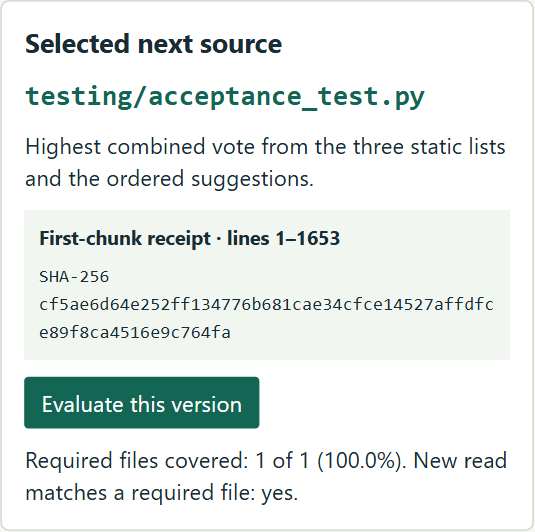
\includegraphics[width=.94\linewidth]{session-read.png}\end{minipage}
\hfill
\begin{minipage}[c]{.62\textwidth}\centering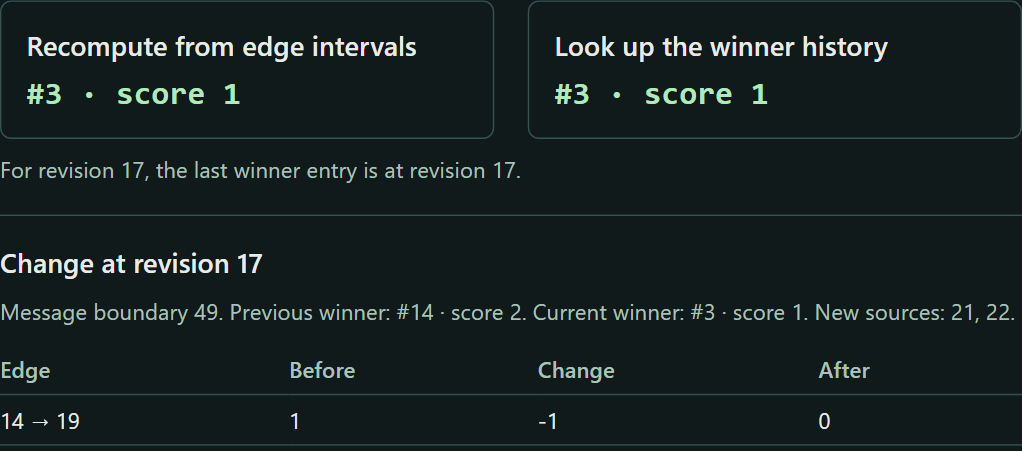
\includegraphics[width=\linewidth]{withdrawal.png}\end{minipage}
\caption{Live SQLite consoles. Left, the committed file read in the pytest session exposes its first-chunk receipt and the result of a separately requested evaluation. Right, the q11 witness table displays the withdrawn support for producer 14. Both historical read plans identify producer 3 at revision 17.}
\label{fig:main}
\end{figure*}

\textit{Cross an import-graph commit.} Open the tox replay and step to commit \texttt{62bd8cf9}. Inspect the eighth-ranked file before and after its score changes. Compare the upper bound on omitted rows with the guaranteed prefix under the published policy. Switch the reserve from 8 to 12 and inspect each policy's indexed reads and returned rows.

\textit{Spend one extra file read.} Choose an archived strict-context session. The first version contains files the agent actually opened, accompanied by a separate list of paths suggested in its final action. Compare the next address proposed from this memory with the address obtained by fusing path-aware lexical, RepoMap and embedding ranks. Commit the selected read (Fig.~\ref{fig:main}) and inspect its line range and digest. The evaluation control now reports whether it added an uncovered relevant file. Return to the earlier version, change the policy, and repeat with the identical one-read budget. Serving and evaluation use distinct SQLite files. For example, on one pytest session the three static rankings plus the ordered proposal list select the previously unopened \texttt{testing/acceptance\_test.py}. The receipt identifies lines 1--1653 of the released first chunk. With evaluation enabled, this read covers the single required file. On that session the first proposal alone loses to three-way static fusion. Two Tokio sessions expose opposite outcomes for suggestion versus static fusion.

\textit{Withdraw support and rewind.} In trace q11 commit through revision 17, then set the read revision to 16. Producer 14 leads with score 2 over producer 3 with score 1. Advance the read revision by one. The witness for edge $14\to19$ records a change from 1 to 0. Producer 14 now also scores 1 and producer 3 wins the tie. Both the interval plan and the winner journal display their SQL plan and result. Rewinding the requested version restores producer 14 without changing the committed horizon.

\textit{Follow a code edit.} Select a line shift and replay the next version. The 315-byte packet survives. An overlapping replacement leaves only 74 of 507 bytes. On a third edit all 14 block IDs survive, yet a snapshot audit exposes three incorrect line addresses in the original display. In the interior-lines example, changing from range invalidation to local alignment restores both blocks. Visitors can examine the addresses and invoke the verifier after each policy change (Fig.~\ref{fig:edit}).

\begin{figure}[t]
\centering\includegraphics[width=.97\columnwidth]{edit.png}
\caption{The code-edit console displays a packet before and after an edit. Its verifier compares address and content in the recorded snapshots even when selected IDs coincide.}
\label{fig:edit}
\end{figure}

\textit{Inspect a packet dependency.} With 2,048 tokens in q02, removing a selected source replaces unit 11 with unit 19 and still covers all 60 annotated characters. In q07, loss of the prefix boundary permits exact reuse. Other controls replay streaming updates, adjust two weights jointly and address Wikipedia documents. All run offline.

\section{Measurements and limits}
\subsection{Maintenance under observed changes}
We replayed 1,072 atomic revisions from 40 ISETrace trajectories. The benchmark executes tools for synthetic OS-agent tasks~\cite{ise,wang}. From changes in their recorded dependencies we obtained 464 net nonzero edge operations, including 118 negative deltas. The single-winner journal matched fresh reconstruction at all 1,112 states, including initial states. It stored 227 records. At eight historical reads per update, the all-candidate version index took $1.34\times$ the time of the journal (paired 95\% interval $[1.29,1.39]$). Raw edge intervals were faster when no historical reads were requested.

For top-$k$, each of five physical plans returned identical IDs and scores for three values of $k$ at all 1,112 states after reopening the database. Membership intervals avoided recording 952 within-list rank moves but still required 717 opens and 398 closes. Packed snapshots had the lowest mean elapsed time at eight reads per update (Table~\ref{tab:top}). The ratio for membership intervals versus snapshots was $1.24$ ($[1.11,1.40]$ over seven paired timing blocks). Rank blocks reduced stored payload from 6,784 to 4,244 bytes, yet both complete checkpointed databases occupied 180\,KiB. These warm local measurements bound the result to small $k$, this change distribution and one machine.

With that packed history fixed, the certificate issued 39 full-index queries across 1,072 updates, versus 533 with unchanged-result detection and 1,072 with unconditional reads. Forty initial reads were common to every plan. The certificate retained 539 unchanged lists and reconstructed 494 changed lists locally. The resulting histories agreed on every ID and score. Warm mixed-workload times were 167.09 versus 165.11\,ms for certificate and unchanged-result control, respectively. For a memory cap of eight pairs, we also retain an upper bound on the best omitted (score, tie key). After a signed update, the cached prefix still above that bound is certified. We fetch only its missing suffix. The variable-length exact prefix of Yi et al.~\cite{topk} provides a matched baseline with indexed suffix refills. Our cache issued 36 warm probes retrieving 38 rows versus 39 probes retrieving 41. Only three of 40 streams differed (paired saving 0.28 probes per 100 updates, interval $[0.00,0.65]$). At capacity nine both required six probes and 12 rows. At twelve both required zero, with mean occupancy 10.08 pairs for ours and 9.94 for the baseline. Eager maintenance of the entire top twelve used 32 probes. Every plan produced the same 533 snapshots. These reserve comparisons measure logical work.

As an external check we replayed import-graph changes over 714 consecutive Git transitions in six Python repositories. Only 56 transitions changed a candidate or edge. At capacity eight the bounded method issued zero warm probes and the published-prefix adaptation issued one, retrieving one row. Each read 48 rows for the initial load across six repositories. The single difference was in tox: support for the eighth file fell from 30 to 29 and the stored outsider bound still certified its rank. At capacity twelve both used zero warm probes and read 72 initial rows. For this workload a saved lookup was rare.

On 108,204 hypothetical source exclusions with fixed costs, scores and rank, the packet criterion identified all 73,261 unchanged packets. On 2,528 single exclusions, the sufficient index approved 2,041 reuses and missed only three. Full recomputation took $5.16\times$ certificate-based serving time ($[4.36,6.17]$ by trajectory) with precomputed features. On 2,000 held-out ISETrace queries under two checkpoint protocols, optimal suffix packing gained 1.88 and 2.04 points in complete annotated support over native first-fit, and $+0.07$ and $-0.04$ against utility-sorted first-fit.

\subsection{How far does this transfer to code?}
On Handoff Debt~\cite{handoff} we calibrated the coordinate guard on 24 issues and evaluated 1,071 observed edits on 13 other issues. Local alignment preserved 323 complete packets versus 302 for range invalidation, an issue-macro difference of 1.97 points ($[1.02,3.03]$). All 29,713 mapped lines matched the snapshots. Common ends alone preserved 322 packets. The supplied edit strings totaled 1.22\,MB, compared with 141.18\,MB for the complete version pairs. Given both whole versions, range plus unique-content validation preserved 341 packets. Only 69 subsequent reads had an informative uncensored window: local alignment covered six completely versus four for ranges. Preserving a larger packet need not change a future action.

\balance
We evaluated a proposed next read on 283 archived GPT-5.4-mini sessions in 25 repositories from Agent Retrieval Bench~\cite{arb}. All arms retain the same strict context, exclude files already read and can add one file. The candidate is the first eligible explicit suggestion, falling back to three-way reciprocal rank fusion when the proposal supplies no such address. For each static list, fusion adds a vote of $1/(60+r)$ at original rank $r$. A hit means the additional read actually adds an uncovered reference file. A chunk witness validates the address before evaluation. The agent's explicit unread-file proposal yielded 20 hits, a fusion of three published rankings 16, and the published Qwen3-Embedding-4B ranking alone 26. The proposal won 15 cases and lost 11 against fusion, a difference of 1.41 points (repository bootstrap 95\% interval $[-2.06,3.80]$). In 48 sessions a proposed list contained some relevant new file. In a second comparison both policies had four lists: adding suggestions as the fourth list versus adding Qwen3-Embedding-8B produced nine gains and eight losses, or $+0.35$ points $[-2.93,3.18]$. The proposal field was identified in a schema audit after the initial registered field rarely contained an eligible path. These results concern a read policy applied to finished sessions. The released ranks arrive precomputed. The comparison prices one additional read and leaves index construction and a fresh agent trajectory outside the measurement.

Two controls test the broader hypothesis that visible dependencies automatically improve context quality. On 54 real \emph{edit2ripple} tasks from ten repositories~\cite{arb}, matching changed symbols with a direction-compatible import or package scope attained 33.49\% mean file Recall@5, versus 33.02\% with matched name evidence. Both arms fuse ranks and exclude the supplied edited file. Under the same filtering the released path-aware lexical rank attained 48.92\%, and RepoMap 44.60\%. The reported metric averages the fraction of each task's reference files retrieved. These are adaptation results on the same 54 tasks.

For an executable check, we masked one method in a ClassEval program~\cite{classeval}. We supplied Qwen3-4B-Instruct-2507 (Q4\_K\_M, greedy decoding) with a visible caller body or an equally long BM25 snippet and ran the generated method against the released tests. At 384 output tokens the counts passing all tests were 41/61 with the caller, 42/61 with BM25 and 41/61 with no neighbor body. The first two choices agreed on the input address 50 times. A follow-up prompted by a truncated generation raised the cap to 768 tokens. All arms then passed 43/61. This method-completion pilot across 32 classes measures executable correctness on an adapted task. The clearest evidence for using these graph views is consequently exact, auditable maintenance under change. End-to-end issue resolution remains open.

\section*{Acknowledgments}
OpenAI Codex drafted Sections I--IV, implemented the views in Section II, generated the interactive demonstration and figures in Section III, and ran and analyzed the experiments in Section IV. Measurements were checked against saved per-query, per-edit and timing records.
\bibliographystyle{IEEEtran}
\bibliography{sources}
\end{document}
